\documentclass[landscape]{foils}
\usepackage[pdftex]{color}
\usepackage[pdftex]{graphicx}
\usepackage{eso-pic}
\usepackage[top=2cm, bottom=2cm, outer=0cm, inner=0cm]{geometry}
\usepackage{listings}
\usepackage{amsmath}
\usepackage{fancyvrb}
\usepackage{xcolor}


\DeclareMathOperator{\sign}{sign}

% colors
\definecolor{DarkRed}{rgb}{0.5,0.0,0.0}
\definecolor{DarkBlue}{rgb}{0.0,0.0,0.35}
\definecolor{DarkGreen}{rgb}{0.0,0.6,0.00}
\definecolor{Orange}{rgb}{0.70,0.30,0.0}
\definecolor{Magenta}{rgb}{0.8,0.0,0.8}
\definecolor{DarkGray}{rgb}{0.3,0.3,0.3}
\def\red{\color{red}} 
\def\darkred{\color{DarkRed}} 
\def\blue{\color{DarkBlue}} 
\def\green{\color{DarkGreen}} 
\def\orange{\color{Orange}}
\def\magenta{\color{Magenta}}
\def\black{\color{black}}
\def\gray{\color{DarkGray}}

% sizes, footer and headers
\textwidth = 26truecm
\textheight = 18truecm
\topmargin =-2 cm
\oddsidemargin -1.5cm
\rightfooter{}
\MyLogo{\darkred {\bf QE-2019}: Summer School on Advanced Materials
  and Molecular Modelling}
%
\def\indent{\hspace*{1cm}}
\def\prompt{\texttt{\$~}}
\def\exec#1{\indent\prompt\code{#1}}
\def\codeline#1{\indent\code{#1}}
\parindent 0pt

% alias for slides header
\def\Head#1{\foilhead{\red #1 \vskip -1cm} \medskip\hrule\medskip}
\def\head#1{\foilhead{\red #1 \vskip -1cm}}

% aliases for codes, files, namelists, etc.
\def\codecolor{\green}
\def\cardcolor{\orange}
\def\code#1{\texttt{\codecolor #1}}
\def\prog#1{\texttt{\red #1}}
\def\var#1{\texttt{\red #1}}
\def\file#1{\texttt{\green #1}}
\def\cmd#1{\texttt{\green #1}}
\def\nml#1{\texttt{\magenta #1}}
\def\card#1{\texttt{\cardcolor #1}}
\def\flag#1{\texttt{\green #1}}

% aliases for math
\def\vr{\ensuremath{\bm{r}}}
\def\vR{\ensuremath{\bm{R}}}
\def\vk{\ensuremath{\bm{k}}}
\def\vtau{\ensuremath{\bm{\tau}}}


\begin{document}
\AddToShipoutPictureBG*{
\includegraphics[width=\paperwidth,height=\paperheight]{figs/qe2021-background-4x3.png}}

\blue
%
\includegraphics[width=1.0\textwidth]{figs/QE2019-logo.pdf}
~\\
\vspace*{4cm}
\MyLogo{~}
\vspace{5em}
\begin{center}
  {\burgundy\LARGE\bf QE-2021: Hands-on session -- Day-7}\\[2em]
  {\burgundy\LARGE (Magnetism in transition metals )}
  ~\\[1.5em]  
  \large Pietro Delugas, Alessandro Stroppa, Sukanya Ghosh, \\
	Nandhakumar Velankanni, Subrahmanian Sappati, Lei Qiao\\
  
\end{center}

%%%%%%%%%%%%%%%%%%%%%%%%%%%%%%%%%%%%%%%%%%%%%%%%%%%%%%%%%%%%% 
\Head{QE-2021: Hands-on session -- Day-7}
\MyLogo{\burgundy {\bf QE-2021}: MaX School on Advanced Materials and Molecular Modelling}
\rightheader{\hspace{-0.8cm}
\includegraphics[width=4.5cm]{figs/QE.png}}
Topics of Day-7 hands-on session:
\begin{enumerate}
	\item Comparison of magnetic and non-magnetic solution for Fe (bcc) (\file{exercise1.ferromagnetic\_vs\_nonmagnetic/})
	\item Dependence of exchange splitting on the lattice constant. \\ (\file{exercise2.volume\_dependence})  
	\item Comparison of \emph{3d} occupations in transition metals (Fe, Co, Ni) (\file{exercise3})  
	\item Plotting bands of magnetic material collinear and non collinear case. (\file {exercise4.bands}) 
\end{enumerate}
   
%%%%%%%%%%%%%%%%%%%%%%%%%%%%%%%%%%%%%%%%%%%%%%%%%%%%%%%%%%%%%
\head{How to run calculations remotely on the ``hpc'' HPC cluster}
\rightheader{}

Several utility commands have been implemented specially for the
QE-2021 school to aid at submitting jobs to HPC cluster(s). These are:
{\small
\begin{itemize}
\item \cmd{\bf remote\_mpirun} -- this is like \cmd{mpirun}, but it
  automatically submits the calculation to a queuing system on the
  ``hpc'' HPC system. For example, a \prog{pw.x} calculation can be
  submitted
  as:\\[0.5em]
  \exec{remote\_mpirun pw.x -in pw.file.in}\\[0.5em]
  where \file{pw.file.in} is the name of the \prog{pw.x} input
  file. {\bf BEWARE:} stdin/stdout redirection does not work for
  \cmd{remote\_mpirun}, hence you must use \flag{-in} (or \flag{-inp})
  option (i.e., do note use ``\cmd{<}'' redirection operator). You do
  not need to specify the number of processors, because the default is
  set to \flag{-np~20}.

  A different number of processors, say 8, can be requested
  as:\\[0.5em]
  \exec{NPROC=8 remote\_mpirun pw.x -in pw.file.in}  
  \vspace{0.5em}
  
\item \cmd{\bf remote\_pwtk} -- this automatically submits the PWTK
  script to queuing system on the ``hpc'' HPC system. Example:\\[0.5em]
  \exec{remote\_pwtk script.pwtk}\\[0.5em]
  where \file{script.pwtk} is the name of the PWTK script.
  \vspace{0.5em}
\clearpage
\item \cmd{\bf remote\_sbatch} -- automatically submits the Unix-shell
  script to queuing system on the ``hpc''  HPC system. Examplee:\\[0.5em]
  \exec{remote\_sbatch script.sh}\\[0.5em]
  where \file{script.sh} is the name of the Unix-shell script.
  When you run in the HPC cluster use increase the number of pools
  change  the line: 
        \vspace{0.5em}
	\begin{Verbatim}[commandchars=\\\{\}]
	mpirun -np $NPROC $PW  < fe.scf.$latt.in -nk 2   >  fe.scf.$latt.out
	\end{Verbatim}
  in 
	\begin{Verbatim}[commandchars=\\\{\}]
	mpirun -np $NPROC $PW  < fe.scf.$latt.in \textcolor{red}{-nk 10}  >  fe.scf.$latt.out
	\end{Verbatim}
	        
  \vspace{0.5em}

\item \cmd{\bf remote\_squeue} -- this checks the status of the job in the queuing
  system on the ``hpc'' HPC system. Example:\\[0.5em]
  \exec{remote\_squeue}
  {\green\burgundy
    \begin{verbatim}
        JOBID PARTITION     NAME     USER ST       TIME  NODES NODELIST(REASON)
     26098354       all submit.n    qe001  R       0:27      1 wn150
\end{verbatim}}
    Where status (ST) R stands for running and PD for pending.
  \vspace{0.5em}
  
\item \cmd{\bf hpc} -- this makes \cmd{ssh} to ``hpc'' HPC login node,
  such that the user will be located in the same directory as used
  locally
  \vspace{0.5em}
  
\item \cmd{\bf rsync\_to\_hpc} -- copies specified files to the
  ``hpc'' cluster to the same directory as is currently
  used locally. Example:\\[0.5em]
  \exec{rsync\_to\_hpc '*.in'}\\[0.5em]
  This will copy all \file{*.in} files from local directory to the
  same directory on the ``hpc'' cluster, whereas:\\[0.5em]
  \exec{rsync\_to\_hpc .}\\[0.5em]
  will copy all the files in the current directory to the same
  directory on the ``hpc'' cluster.
  \vspace{0.5em}
  
\item \cmd{\bf rsync\_from\_hpc} -- download the specified file from
  the ``hpc'' cluster from the same directory as is
  currently used locally. Example:\\[0.5em]
  \exec{rsync\_from\_hpc '*.out'}\\[0.5em]
  This will copy all \file{*.out} files from the ``hpc'' cluster to
  the local host (virtual machine).
\end{itemize}
}
%%%%%%%%%%%%%%%%%%%%%%%%%%%%%%%%%%%%%%%%%%%%%%%%%%%%%%%%%%%%% 
\head{Exercise 1: Task 1 }
\rightfooter{Exercise 1: Compare magnetic and non magnetic ground states} 
\begin{itemize}
	\item Compare the magnetic and the non-magnetic solution for Fe (bcc) 
	\item {\bf Find the optimized lattice constant for non-magnetic Fe (bcc)}:
		\begin{enumerate}
			\item go to {\small \file{exercise1.ferromagnetic\_vs\_nonmagnetic/non\_magnetic}
      }:
		
			\item Use the scripts {\small \file{job.sh}} or {\small \file{job.pwtk}} 
      to scan the lattice constants from $4.6~\mathrm{Bohr}$ to  $5.9~\mathrm{Bohr}$. 
			\item use \code{ev.x} to fit the data collected in \file{energies.dat}  with the 
          Murnaghan EOS and find the optimized lattice constant.
		\end {enumerate}
  \item {\bf Find the optimized lattice constant for magnetic Fe (bcc)}
      \begin{enumerate}
        \item go to {\small \file{~/Day-7/exercise1.ferromagnetic\_vs\_nonmagnetic/magnetic}}
        \item repeat steps 2 and 3 as for the non-magnetic case. 
      \end{enumerate}
  \item {\bf Plot and compare energies and lattice constants}
      \begin{itemize}
        \item go to {\small \file{~/Day-7/exercise1.ferromagnetic\_vs\_nonmagnetic/}}
        \item use the gnuplot script \file{compare.gp} to plot your results. 
      \end{itemize}
\end{itemize}



%%%%%%%%%%%%%%%%%%%%%%%%%%%%%%%%%%%%%%%%%%%%%%%%%%%%%%%%%%%%%%%%%%%%%%%%%%%%%%%%%%%%%%
\Head{Compare energies and lattice constants.}
\vfill
\parbox{10cm}{
  \begin{itemize}
    \item The magnetic solution has a lower total energy per cell. 
    \item The magnetic solution has a larger lattice constant than the non-magnetic. 
    \item LSDA underestimate lattice constant $\sim 5.2~\mathrm{Bohr}$ vs. $\sim 5.4~\mathrm{Bohr}$ 
    of the experiment.  
  \end{itemize}
}
\hfill \parbox{14cm}{
  \begin{center}
    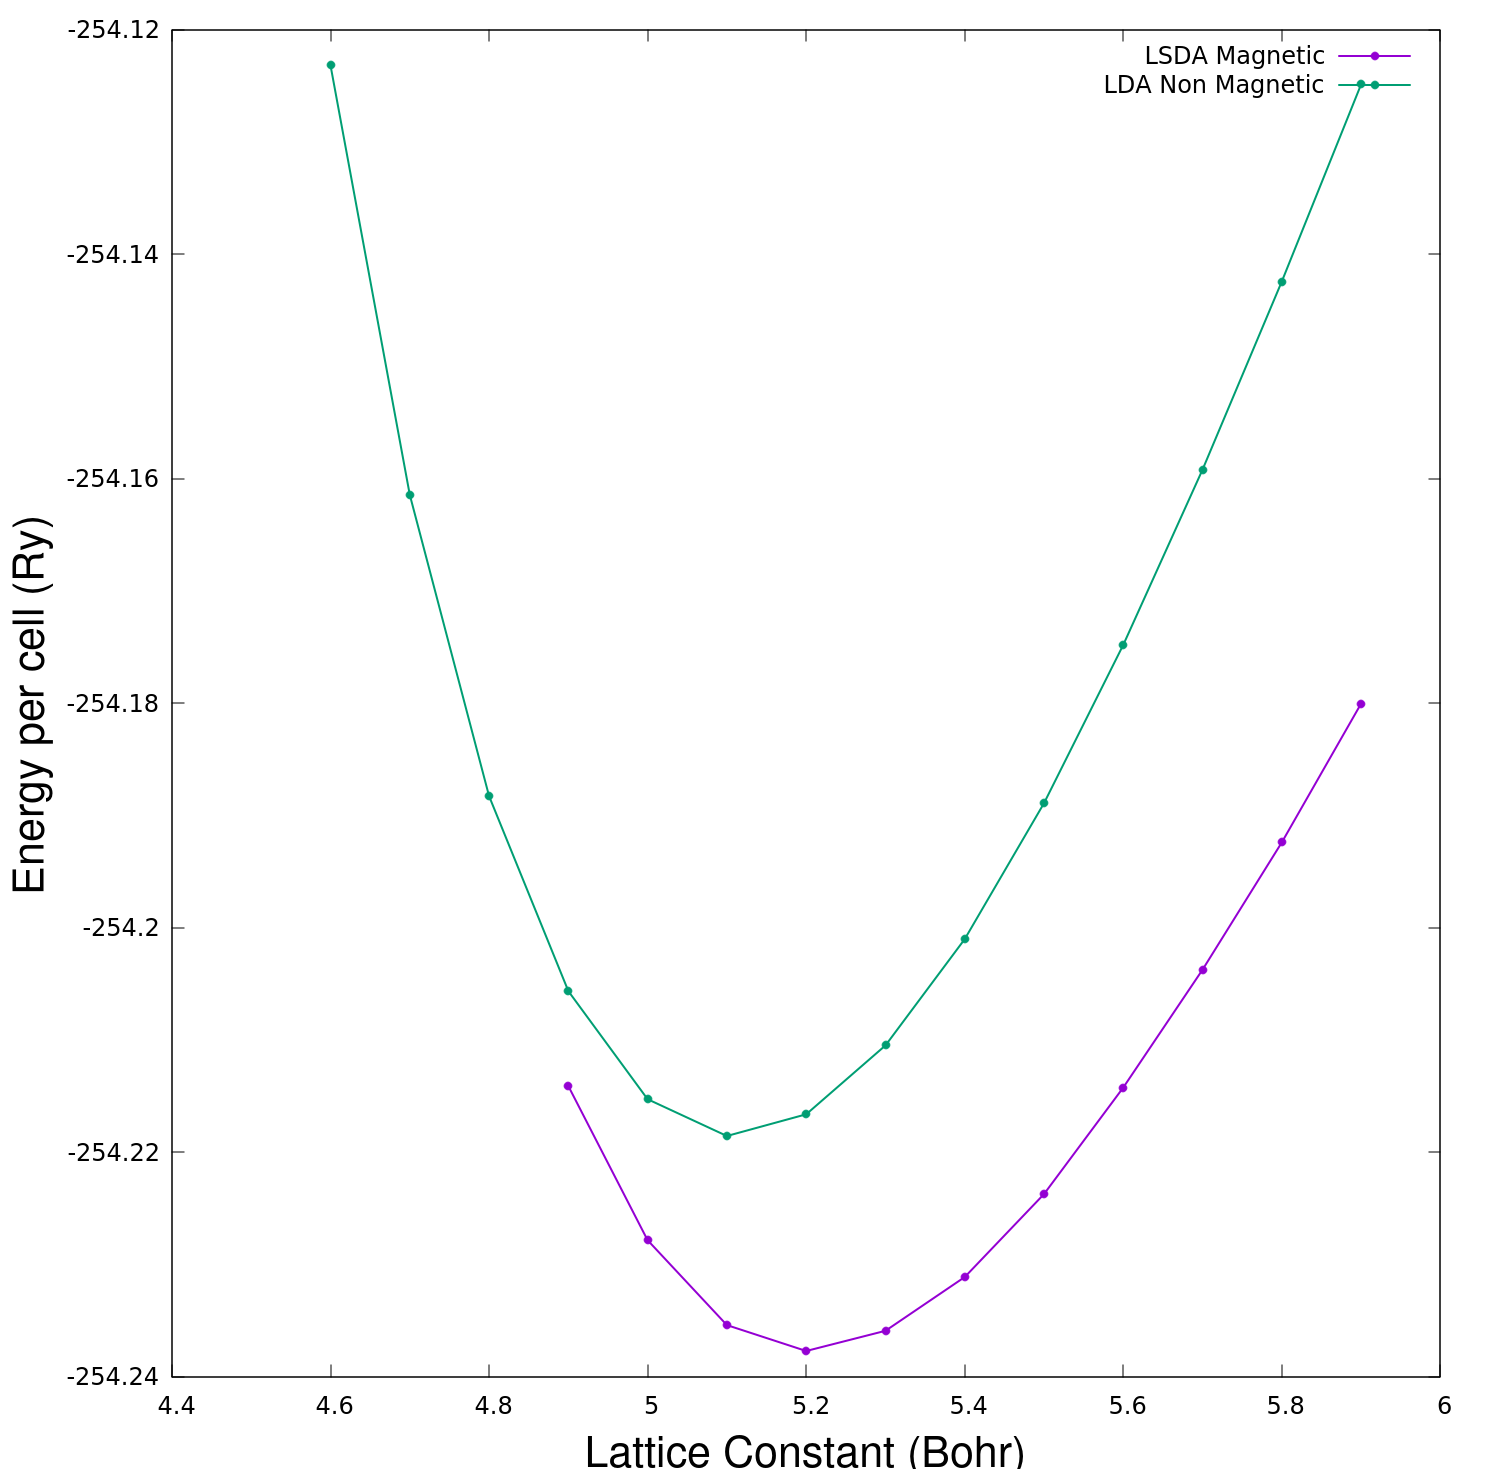
\includegraphics[width=13.5cm]{figs/alat_lda_mag_vs_mag.png}\\
  \end{center}
}
\vfill

%%%%%%%%%%%%%%%%%%%%%%%%%%%%%%%%%%%%%%%%%%%%%%%%%%%%%%%%%%%%%%%%%%%%%%%%%%%%%%%%%%%%%
\Head{Remarks on input}
How to select the magnetic solution: 

\begin{minipage}{11cm}
 \small{
 \begin{Verbatim}[frame=single, commandchars=\\\{\}]
&system
  ibrav=3, 
  celldm(1)=$latt, 
  nat= 1, 
  ntyp=1,
  \textcolor{red}{nspin=2},  
  \textcolor{red}{starting_magnetization(1)=0.3},
  ecutwfc=70.0, ecutrho=850.0,
  occupations='smearing', 
  smearing='marzari-vanderbilt', 
  degauss=0.02
/
 \end{Verbatim}
 }
\end{minipage}\hspace{1em}
\parbox{12cm}{
  \begin{itemize}
    \item {\ttfamily \small nspin=2} Specify  the spin polarized calculation.
    \item To allow a magnetic solution we have also break the symmetry between the \emph{up} 
      and \emph{down} channel:
      \begin{itemize} 
        \item {\ttfamily \small starting\_magnetizion(1)=0.3} Builds the starting potential assuming 
          an initial  magnetization of Fe of $0.3 \times 16$.
      \end{itemize}
    \end{itemize}
}
\Head {Remarks on input}
Magnetic system in the non-collinear case 


\begin{minipage}{11cm}
  \begin{Verbatim}[frame=single, commandchars=\\\{\},fontsize=\small]
&system
  ibrav=3
  celldm(1)=5.4,
  nat=1,ntyp=1,
  \textcolor{red}{noncolin=.true.},
  \textcolor{red}{starting_magnetization=0.3},
  \textcolor{red}{angle1(1)=0.0},
  \textcolor{red}{angle2(1)=0.0},
  ecutwfc=70.0,
  ecutrho=850.0,
  occupations='smearing', 
  smearing='marzari-vanderbilt', 
  degauss=0.02
/
  \end{Verbatim}
\end{minipage}
\hfill \parbox{14cm}{
  \begin{itemize}
    \small
    \item non-collinear case is selected specifying \var{noncolin=.true.}
    \item \var{starting\_magnetization} must be specified for at least one species otherwise the
      program will perfom a non-magnetic calculation.
    \item in the non-collinear case magnetization is a vector, it is possible to specify the direction of 
      the starting magnetization for each atomic type:
      \begin{itemize}
        \item \var{angle1}  is the  angle with the  $z$ axis (in degrees);
        \item \var{angle2}  is the  azimuthal angle (in degrees)
      \end{itemize}
  \end{itemize}
}
%%%%%%%%%%%%%%%%%%%%%%%%%%%%%%%%%%%%%%%%%%%%%%%%%%%%%%%%%%%%%%%%%%%%%%%%%%%%%%%%%%%
\Head{How the magnetization is reported in output}
\begin{itemize}
  \item In the spin-polarized case the total magnetization is reported at each SCF step
    and at the end of the calculation: 
    \begin{Verbatim}[frame=single,fontsize=\small]
      total magnetization       =     2.22 Bohr mag/cell
      absolute magnetization    =     2.28 Bohr mag/cell
    \end{Verbatim}
  \item In the magnetic non-collinear case:
    \begin{Verbatim}[frame=single,fontsize=\small]
      total magnetization       =     1.38     0.00     1.38 Bohr mag/cell
      absolute magnetization    =     1.99 Bohr mag/cell
    \end{Verbatim}
  \item An estimate of the magnetization at each ionic site is also printed at the end of the calculation
    \begin{Verbatim}[frame=single, fontsize=\small]
      Magnetic moment per site  (integrated on atomic sphere of radius R)
      atom   1 (R=0.357)  charge= 14.4267  magn=  2.2287
    \end{Verbatim}
  \item In the magnetic non-collinear case:
    \begin{Verbatim}[frame=single, fontsize=\small]
     atom number    1 relative position :    0.0000   0.0000   0.0000
     charge :    14.332507  (integrated on a sphere of radius 0.357)
     magnetization :          1.374808   -0.000000    1.374808
     magnetization/charge:    0.095922   -0.000000    0.095922
     polar coord.: r, theta, phi [deg] :     1.944273   45.000000   -0.000000
    \end{Verbatim}
\end{itemize}
%%%%%%%%%%%%%%%%%%%%%%%%%%%%%%%%%%%%%%%%%%%%%%%%%%%%%%%%%%%%%%%%%%%%%%%%%%%%%%%%%%%
\Head{Input of \code{dos.x} and \code{projwfc.x}}
\begin{minipage}{14cm}
  \begin{Verbatim}[frame=single, commandchars=\\\{\},fontsize=\small]
    &dos
      prefix='fe',
      bz_sum='tetrahedra_opt'
      Emin=5.0
      Emax=25.0 
      DeltaE=0.05
      fildos='fe.dos'
    /
  \end{Verbatim}
\end{minipage}
\hfill
\parbox{12cm}{
  \begin{itemize}
    \small
    \item \var{bz\_sum} selects the integration method. 
    \item \var{Emin},\var{Emax}, and \var{DeltaE} define the range and definition of the DOS;
    \item to select the range first use default values, then select the right window
  \end{itemize}
}
\vfill 
\begin{minipage}{14cm}
  \begin{Verbatim}[frame=single, commandchars=\\\{\},fontsize=\small]
 &projwfc
    !outdir='./tempdir/',
    prefix='fe'
    Emin=5.0, Emax=25.0, DeltaE=0.05
 /
  \end{Verbatim}
\end{minipage}
%%%%%%%%%%%%%%%%%%%%%%%%%%%%%%%%%%%%%%%%%%%%%%%%%%%%%%%%%%%%%%%%%%%%%%%%%%%%%%%%%%%%%%%%%
\Head{Exercise 1: Task 2}
Using the optimized lattice constants obtained in task 1 we analize the electronic 
structures of the  two solutions. 
\begin{enumerate}
  \item Make the SCF and non-SCF computations for boths solutions. 
  \item Compute the  DOS for both solutions
  \item Compute the pDOS for the magnetic solution
\end{enumerate}
\begin{center}
  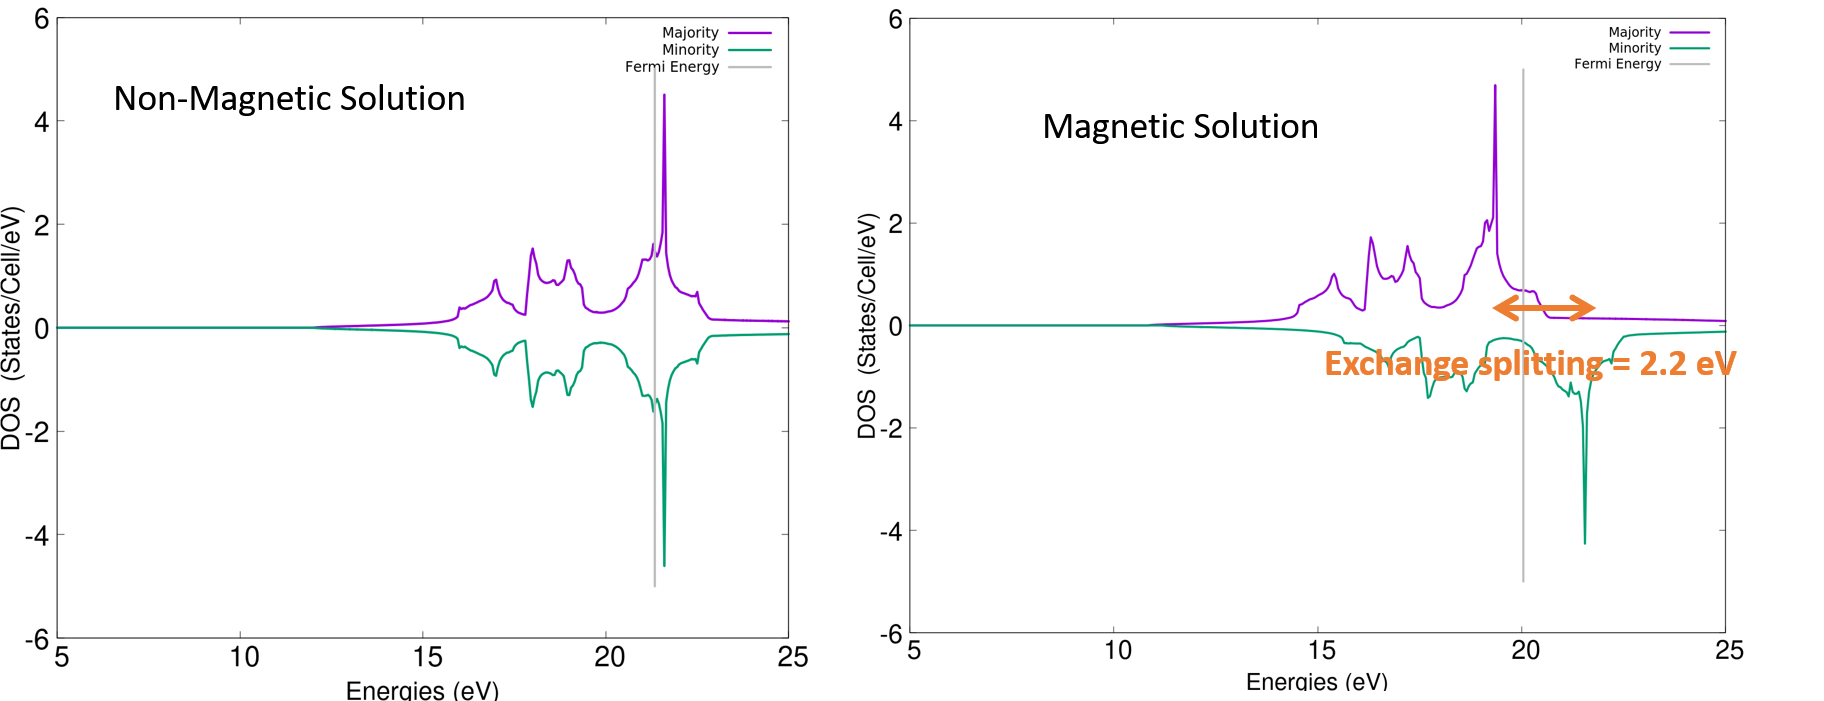
\includegraphics[width=24cm]{figs/mag_non_mag_DOS.png}
\end{center}
%%%%%%%%%%%%%%%%%%%%%%%%%%%%%%%%%%%%%%%%%%%%%%%%%%%%%%%%%%%%%%%%%%%%%%%%%%%%%%%%%%%%%%%%%
\Head{Exercise 2: Magnetization vs. volume}
\rightfooter{Exercise 2. Magnetization vs. volume}
\begin{itemize}
  \item The aim of this exercise is to see how the magnetization and the exchange splitting 
  behaves  when the lattice constant decreases 
  \item Here we use the PBE functional that gives a more realistic lattice constant than LDA. 
  \item The exercise proceeds along  the following steps:
    \begin{enumerate}
      \item Run a script for determining the optimized lattice constant
      \item Use \code{ev.x} to estimate the optimized lattice constant fitting the energies
        to the Murnaghan EOS. 
      \item Use the data in the file \file{magnetization.dat} to see how the magnetization 
        changes when we change the lattice constant. 
      \item {\bf Assignment} Compute the electronic structure for  3 different values of lattice 
      constant and estimate the the exchange splitting as we did in exercise 1. 
    \end{enumerate}
  \end{itemize} 
%%%%%%%%%%%%%%%%%%%%%%%%%%%%%%%%%%%%%%%%%%%%%%%%%%%%%%%%%%%%%%%%%%%%%%%%%%%%%%%%%%%%%%%%%%%%%%%%%%%
\Head{Magnetization vs. alat}
\vfill
\begin{center}
  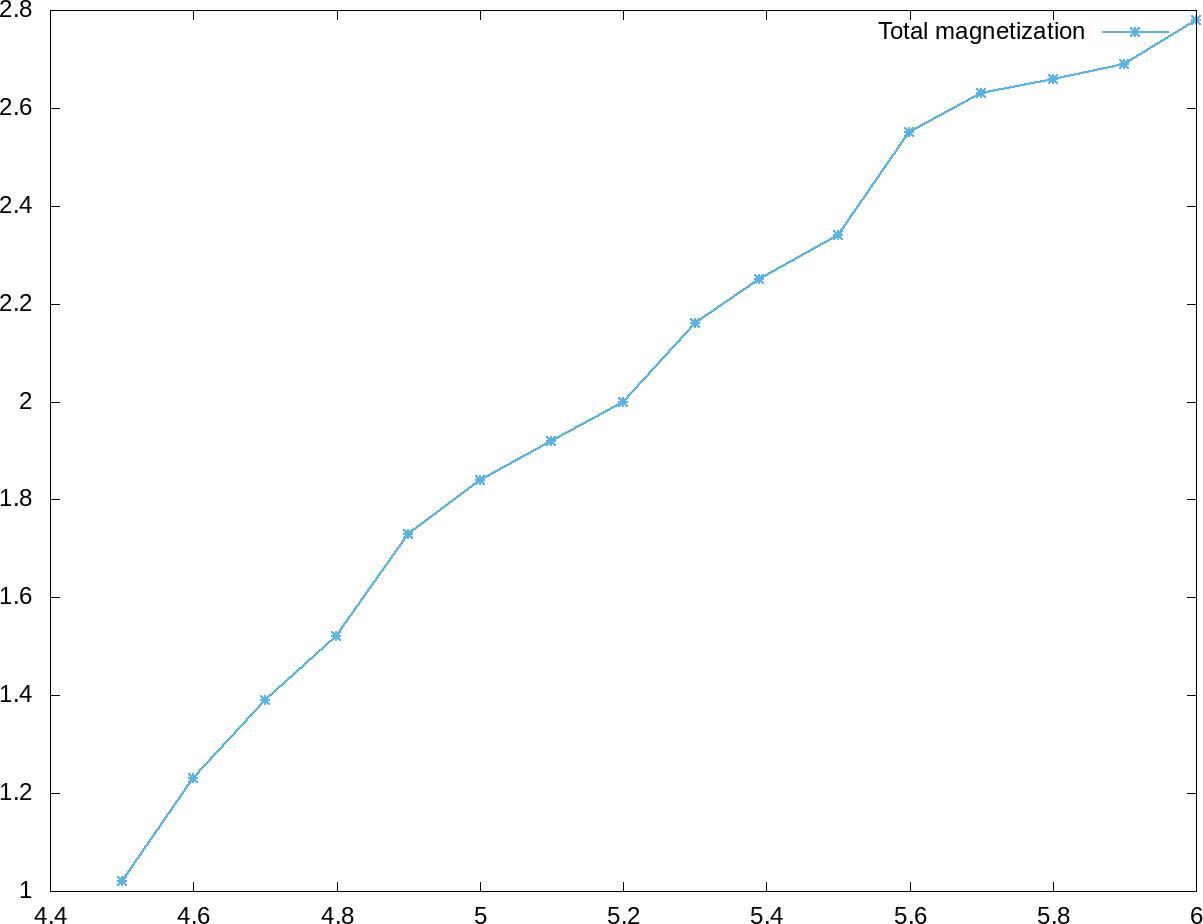
\includegraphics[width=17cm]{figs/mag_v_vol.png}
\end{center}
\vfill
%%%%%%%%%%%%%%%%%%%%%%%%%%%%%%%%%%%%%%%%%%%%%%%%%%%%%%%%%%%%%%%%%%%%%%%%%%%%%%%%%%%%%%%%%%%%%%%%%
\Head{Exercise 3. Comparing magnetization and exchange splitting in transition metals}
  \rightfooter{Exercise 3.}
  In this exercise we compare the magnetic properties of three different 
  transition metals Fe(bcc), Co(hcp), and Ni(fcc)
  \begin{itemize}
    \item With the usual procedure we compute the electronic structure for the  3 transition 
          metals.
    \item use \code{projwf.x} to analize the contribution to the magnetization coming from 
       the different orbitals.
  \end{itemize}
\begin{Verbatim}[fontsize=\small]
  Atom #   1: total charge =  17.0232, s =  2.4486, p =  6.1080, d =  8.4666, 
  spin up      =   8.8345, s =  1.2198, 
  spin up      =   8.8345, p =  3.0211, pz=  1.0070, px=  1.0070, py=  1.0070, 
  spin up      =   8.8345, d =  4.5935, dz2=  0.9308, dxz=  0.9106, dyz=  0.9106, 
                                        dx2-y2=  0.9308, dxy=  0.9106, 
  spin down    =   8.1887, s =  1.2288, 
  spin down    =   8.1887, p =  3.0869, pz=  1.0290, px=  1.0290, py=  1.0290, 
  spin down    =   8.1887, d =  3.8731, dz2=  0.8427, dxz=  0.7292, dyz=  0.7292, 
                                        dx2-y2=  0.8427, dxy=  0.7292, 
  polarization =   0.6457, s = -0.0089, p = -0.0658, d =  0.7204, 
Spilling Parameter:   0.0543
\end{Verbatim}
%%%%%%%%%%%%%%%%%%%%%%%%%%%%%%%%%%%%%%%%%%%%%%%%%%%%%%%%%%%%%%%%%%%%%%%%%%%%%%%%
\Head{Format of \code{projwfc.x} output}
\begin{itemize}
  \item The total DOS and the sum of projected DOS are written to file
  \file{<filpdos>.pdos\_tot}.
  \begin{itemize}
    \item The format for the collinear, spin-unpolarized case and the
    non-collinear, spin-orbit case is:
    \vspace{0.5em}
    \begin{Verbatim}[frame=single,fontsize=\small]
        E DOS(E) PDOS(E)
        ...
    \end{Verbatim}
  
    \item The format for the collinear, spin-polarized case is:
      \vspace{0.5em}
      \begin{Verbatim}[frame=single,fontsize=\small]
        E DOSup(E) DOSdw(E)  PDOSup(E) PDOSdw(E)
        ...
      \end{Verbatim}
    \item The format for the non-collinear, non spin-orbit case is:
      \vspace{0.5em}
      \begin{Verbatim}[frame=single,fontsize=\small]
        E DOS(E) PDOSup(E) PDOSdw(E)
        ...
      \end{Verbatim}

    \end{itemize}
  \end{itemize}
%%%%%%%%%%%%%%%%%%%%%%%%%%%%%%%%%%%%%%%%%%%%%%%%%%%%%%%%%%%%%%%%%%%%%%%%%%%%%%%%%%
\Head{Format of the projection files}
  {\small
  In the collinear case and the non-collinear, non spin-orbit case
  projected DOS are written to file \file{<filpdos>.pdos\_atm\#N(X)\_wfc\#M(l)},
  where N = atom number , X = atom symbol, M = wfc number, l=s,p,d,f
  (one file per atomic wavefunction found in the pseudopotential file)
  }
  \begin{itemize}
    \item The format for the collinear, spin-unpolarized case is:
    \vspace{0.5em}
      \begin{Verbatim}[frame=single,fontsize=\small]
      E LDOS(E) PDOS_1(E) ... PDOS_2l+1(E)
      ...
      \end{Verbatim}

  where 
  \begin{itemize}
    \item LDOS = $\sum_{m=1,2l+1} {PDOS\_{m(E)}}$
    \item PDOS\_m(E) = projected DOS on atomic wfc with component m
  \end{itemize}

\item  The format for the collinear, spin-polarized case and the
  non-collinear, non spin-orbit case is as above with
  two components for both  LDOS(E) and PDOS\_m(E)
  \end{itemize}
%%%%%%%%%%%%%%%%%%%%%%%%%%%%%%%%%%%%%%%%%%%%%%%%%%%%%%%%%%%%%%%%%%%%%%%%%%%%%%%%%
\Head {Orbital order }
\begin{itemize}
\item for l=1:
\begin{enumerate}
  \item $p_z$     (m=0)
  \item $p_x$     (real combination of m=+/-1 with cosine)
  \item $p_y$     (real combination of m=+/-1 with sine)
\end{enumerate}
\item for l=2:
\begin{enumerate}
  \item $d_{z^2}$    (m=0)
  \item $d_{zx}$    (real combination of m=+/-1 with cosine)
  \item $d_{zy}$    (real combination of m=+/-1 with sine)
  \item $d_{x^2-y^2}$ (real combination of m=+/-2 with cosine)
  \item $d_{xy}$    (real combination of m=+/-2 with sine)
\end{enumerate}
\end{itemize}
%%%%%%%%%%%%%%%%%%%%%%%%%%%%%%%%%%%%%%%%%%%%%%%%%%%%%%%%%%%%%%%%%%%%%%%%%%%%%%%%
\Head{Exercise 4: plotting bands}
\rightfooter{Exercise 4: plotting bands}
\begin{itemize}
  \item this exercise provides an example on how to plot the bands of a magnetic system. 
  \item Spin-polarized collinear case:
    \begin{itemize}
      \item \exec {cd Ni\_collinear}
      \item SCF calculation for Ni (bcc): \exec{pw.x < ni.scf.in > ni.scf.out}
      \item non-SCF calculation: 
      \begin{itemize}
        \item \var{calculation='bands'}
        \item set the list of K-points \\
        \\
        \begin{minipage}{12cm}
          \begin{Verbatim}[frame=single, commandchars=\\\{\},fontsize=\small]
K_POINTS crystal_b
6
  0.000  0.000  0.000  20  !gamma
  0.500  0.500  0.500  10  !L
  0.500  0.250  0.750  10  !W
  0.500  0.000  0.500  10  !X
  0.000  0.000  0.000  20  !gamma
  0.375  0.375  0.750  1   !K
          \end{Verbatim}
        \end{minipage}
  \parbox{12cm}{
    \small
    \begin{itemize}
      \item we specify the high-symmetry points and number of points of each segment
      \item \flag{crystal\_b} specify the format for K-points
    \end{itemize}
  }
  \end{itemize}
\item use \code{bands.x} for preparing the band plot and analize symmetry, first for up component 
  then for down component \\


\begin{minipage}{12cm}
   \begin{Verbatim}[frame=single, commandchars=\\\{\},fontsize=\small]
&BANDS
       
  outdir='./tempdir/',
  prefix='ni',
  \textcolor{red}{filband='ni.spinup.band_data'}, 
  \textcolor{red}{spin_component = 1},
/
   \end{Verbatim}
  \end{minipage}
  \hfill
  \parbox{10cm}{
    \small
    \begin{itemize}
      \item \var{spin\_componet} selects the spin component 
      \item \var{filband} selects the prefix where the bands are saved
    \end{itemize}
  }\hfill
  \vskip 1cm

\item the output of \code{bands.x} provides the length of the k-points path and the position 
    of the high-symmetry points 
\item use the gnuplot script to plot the bands
\end{itemize}
\end{itemize}
%%%%%%%%%%%%%%%%%%%%%%%%%%%%%%%%%%%%%%%%%%%%%%%%%%%%%%%%%%%%%%%
\Head{}
\vfill
\begin{center}
  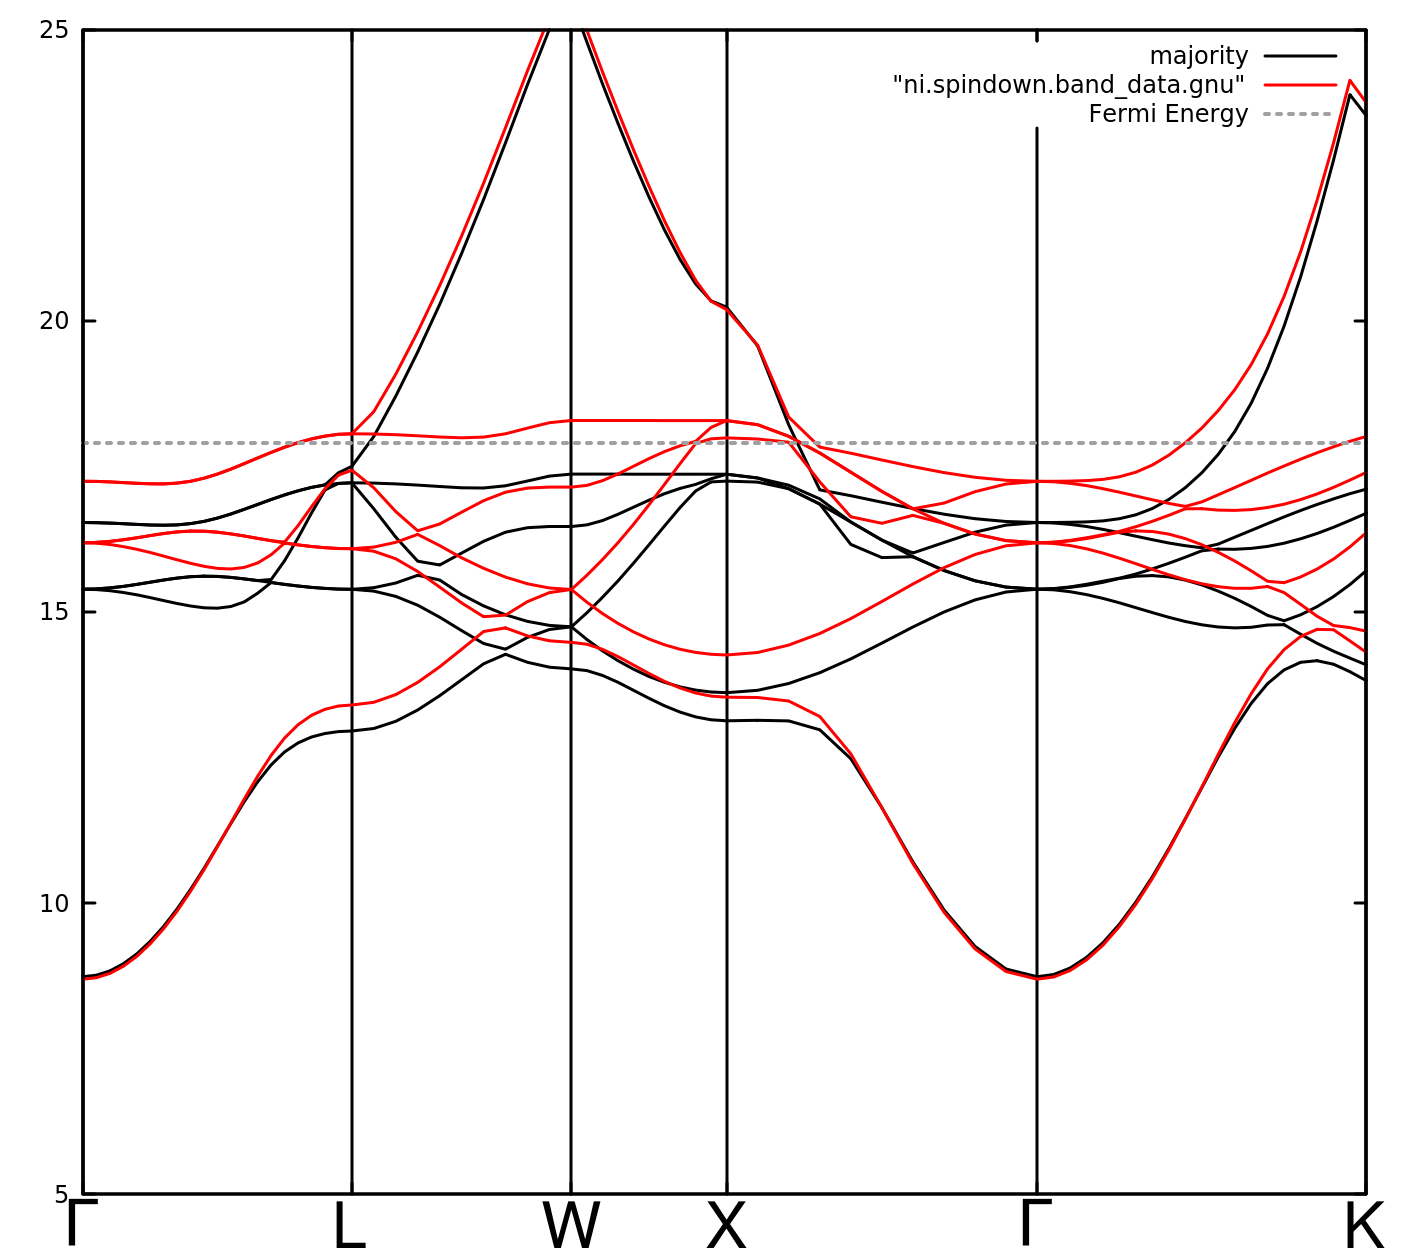
\includegraphics[width=14cm]{figs/bands_Ni_colinear.png}
\end{center}
\vfill
%%%%%%%%%%%%%%%%%%%%%%%%%%%%%%%%%%%%%%%%
\Head{Non-collinear case}
\begin{itemize}
  \item  Plot the Ni bands in the noncollinear case:
  \begin{itemize}
    \item \exec{cd Ni\_noncollinear} 
    \item run the collinear scf  calculation for Ni in this directory:\\
        \exec{pw.x < ni.scf.in > ni.scf.out}
    \item run the non-collinear nscf calculation for the bands
    \begin{itemize}
      \item  \var{spin=2} has been replaced with \var{noncolinear=.true.} \\ 
         \exec{pw.x < ni.bands.in > ni.bands.out} 
    \end{itemize}
    \item run `bands.x` for the noncollinear case: 
    \item  \var{spin\_component} has been removed and we add \var{lsigma(3)=.true.} that instructs 
       the program to compute the expectation value for the z component of the spin operator for each
        eigenfunction and save all values in the file \file{ni.noncolin.data.3}. All values in this case are 
        ceeither 1/2 or -1/2 as expected. 
    \item the program \code{plot\_noncolin\_bands.f90} reads this values and writes them together 
       with the band structure in the file  \file{my\_bands.data}.
       \begin{itemize}
         \item  compile the program: \\
                 \exec{ gfortran -o mino.x plot\_noncolin\_bands.f90 }
         \item  copy \file{ni.noncolin.data.3} to \file{ni.noncolin.data.s} 
         \item run the program \\
                 \exec{./mino.x ni.noncolin.data}
         \item use gnuplot and the script \file{bands\_noncollin.gp} to plot the bands in this case. 
         \item start {gnuplot} and type the command: \\
                \exec{gnuplot> load "bands\_noncollin.gp"} 
       \end{itemize}
    \end{itemize}
\end{itemize}
\begin{center}
  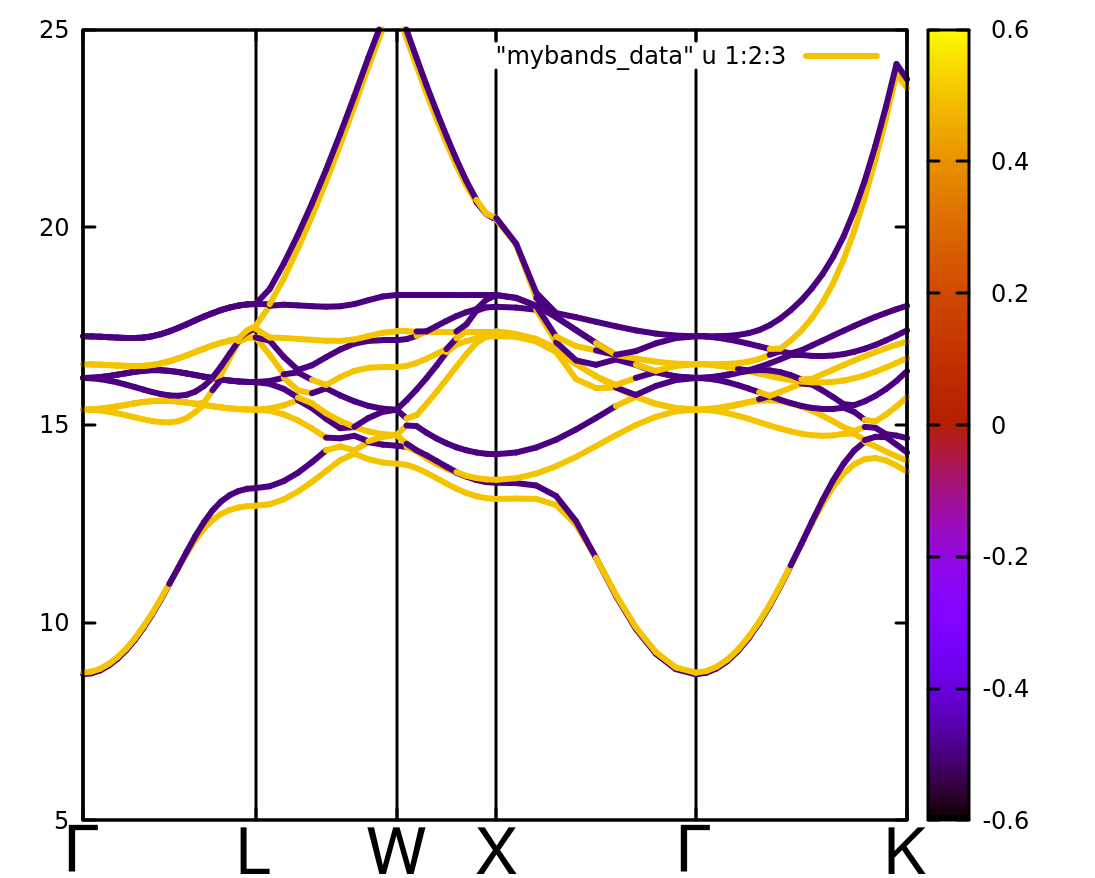
\includegraphics[width=14cm]{figs/bands_noncollinear.png}
\end{center}
\Head{}
\rightfooter{}
\vfill
\begin{center}
  {\Huge \red THE END}
\end{center}
\vfill






\end{document}

%%% Local Variables:
%%% mode: latex
%%% TeX-master: t
%%% End:
